\subsection{Cantidad de paquetes por direcciones IP}

Teniendo las cuatro capturas diferentes sobre redes de diversa índole y, habiendo calculado los respectivos valores de información y entropía (para ambos modelos mencionados previamente, a saber, Modelo Ethernet y Modelo ARP), nos proponemos dar un paso mas y analizar dichos resultados desde varias perspectivas.

En principio, analizaremos cómo la información de cada símbolo de nuestra fuente $S_1$ varía según la cantidad de paquetes ARP (Reply o Request) capturados para cada dirección IP. Para ello recordemos que la fórmula de la Información de un símbolo $s_i \in S_1$ vendrá dada por:

\begin{equation}
 I(s_{i}) = -log_{2}(P(s_{i}))\ bits
\end{equation}

De esta manera, mientras mas elevada sea la probabilidad de ocurrencia del símbolo iésimo, más baja será la información que finalmente nos brindará. De esto podemos inducir que aquellos símbolos cuya información es mucho mas baja que el resto, tuvieron niveles de recurrencia mucho mas altos. Por lo tanto, las direcciones IP que representan habrán concentrado mucho mas tráfico de paquetes ARP que las demas.

Ahora bien ¿Cuanto es poca información? ¿Cuanto es mucho tráfico? Para aclarar dichas dudas debemos utilizar un concepto extra: la entropía, es decir el valor de incertidumbre de la presente fuente. La fórmula de dicho concepto es:

\begin{equation}
 H(S) = \sum_{s \in S} P(s) I(s)
\end{equation}

Así es como podemos vincular y comparar entre sí a cada uno de los valores de información para todo símbolo en la fuente analizada. Para aquellos símbolos cuyos valores de información superen el nivel de entropía, descubriremos que a su vez la cantidad de paquetes ARP relacionados consigo, no superan el promedio. Por el contrario, los símbolos por debajo del nivel de entropía poseen grandes concentraciones de paquetes ARP en su tráfico habitual.

\subsubsection{Red Hogareña}

En la sección anterior, dimos un primer acercamiento a los datos obtenidos en las capturas, mostrando una serie de grafos dirigidos donde los nodos eran las direcciones IPs y los ejes (con peso) eran las cantidades de paquetes ARP que habían transitado entre dos nodos. En dichos gráficos se pudieron ver ciertos nodos que resaltaban del resto por la gran cantidad de paquetes ARP que concentraban. Entonces, por medio del cálculo de la información para cada símbolo, tendremos mas elementos para respaldar nuestras ideas.

\centerline{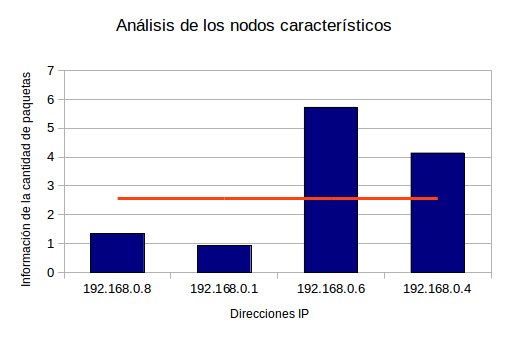
\includegraphics[width=0.9\textwidth]{./graficos/paquetesVSIP/casa_mari.png}}

En el histograma de Información vemos fácilmente como el valor mas bajo es alcanzado por el símbolo correspondiente para la IP 192.168.0.1, que precisamente en el digrafo aparecía como el mas concurrido. Decimos entonces que efectivamente, a dicho símbolo le pertenece la IP mas recurrente en la captura actual, por lo tanto es un nodo distinguido.

\subsubsection{Red Laboratorio}

En este caso, el histograma en principio no nos revela datos contundentes porque el número de hosts en la red es muy grande (supera ampliamente el caso anterior).

\centerline{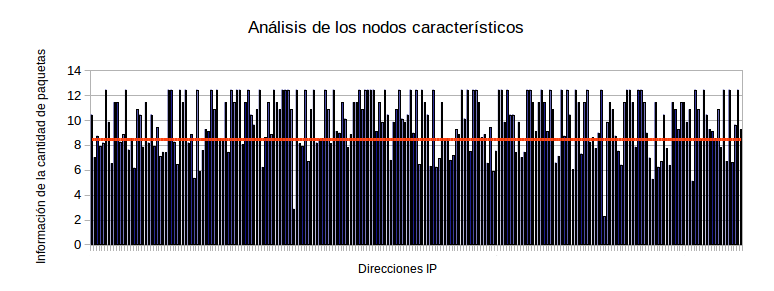
\includegraphics[width=1\textwidth]{./graficos/paquetesVSIP/labo5_muchos.png}}

Es por ello que decidimos filtrar los resultados y mostrar solamente los cincuenta valores de información mas bajos obtenidos por la captura. Esto es así para poder observar con mayor comodidad aquellas direcciones IP que realmente son relevantes para el experimento. Vemos que en particular, todos los valores filtrados quedaron por debajo de la línea de entropía, convirtiendolos en los nodos mas recurrentes de la red.

\centerline{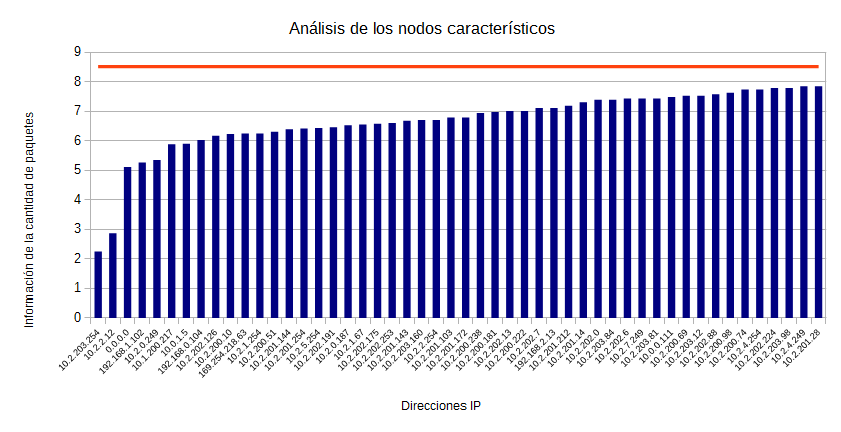
\includegraphics[width=1\textwidth]{./graficos/paquetesVSIP/labo5.png}}

También vemos claramente en el histograma, que la IP 10.2.203.254 le pertenece al nodo mas distinguido. Efectivamente es el mismo nodo que en el digrafo correspondiente habíamos resaltado. Si recordamos la particular disposición del nodo en cuestión en el grafo y hacemos hincapié en la gran diferencia entre la cantidad de información del mismo y los otros símbolos, concluímos que dicha dirección pertenece al \textit{switch} del laboratorio, nodo distinguido por excelencia.

\subsubsection{Red Devartis}

Para esta red no fue necesario realizar ningún tipo de filtrado. Se pueden ver muy fácilmente los valores de información calculados para los diferentes símbolos. Es así como se puede reafirmar la idea que se había planteado en la sección previa: el nodo 192.168.1.1 es el mas distinguido, seguido inmediatamente (pero con bastante diferencia) por el nodo 192.168.1.211.

\centerline{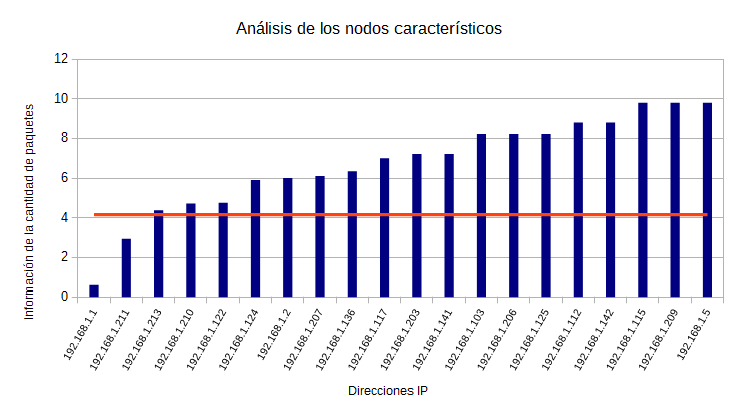
\includegraphics[width=1\textwidth]{./graficos/paquetesVSIP/laburo_mari.png}}

Como se puede apreciar, esos dos símbolos son los únicos que quedaron por debajo de la entropía. Esto refuerza la idea que la cantidad de paquetes ARP que transitaron por ambos nodos es mucho mas grande que la del resto y que hay una gran diferencia de concentración de paquetes entre los dos grupos. Ambos son nodos distinguidos. De no ser así (es decir, si la diferencia y el tránsito no fueran tan grandes), las probabilidades de ocurrencia serían mas similares, al igual que los valores de información. Por lo tanto la entropía sería mucho mas elevada.

\subsubsection{Red Mercap}

Finalmente, en esta red donde habíamos obtenido mucha información en la sección anterior, podemos corroborar y reforzar ciertas ideas que habíamos planteado.

\centerline{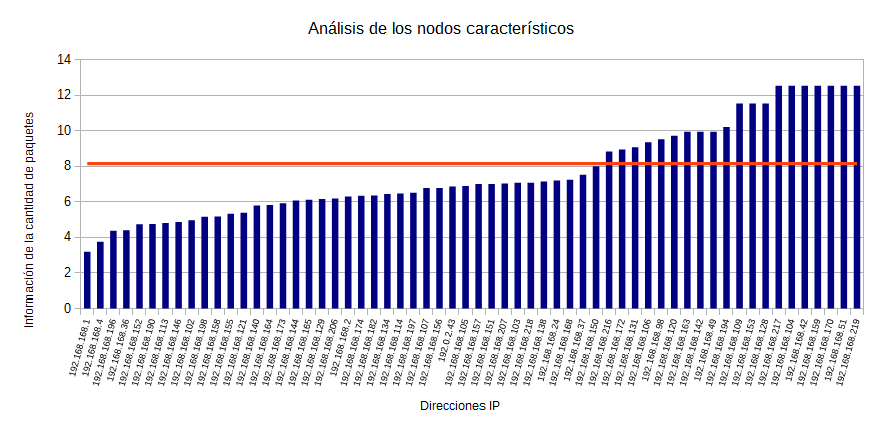
\includegraphics[width=1\textwidth]{./graficos/paquetesVSIP/laburo_eze.png}}

Como podemos ver, todos los nodos que suponíamos eran los distinguidos, aparecen en los primeros lugares del histograma, con los valores de información mas bajos de la captura. Efectivamente, todo apunta que dichos hosts son en realidad los servidores de la empresa. Estos nodos mencionados tienen demasiada presencia en la red, y son recurrentes a la hora recibir o enviar paquetes ARP. Todos indícios de que efectivamente las IPs representan los servidores.